\documentclass[conference]{IEEEtran}
\IEEEoverridecommandlockouts
\usepackage{cite}
\usepackage{amsmath,amssymb,amsfonts}
\usepackage{graphicx}
\usepackage{textcomp}
\usepackage{hyperref}
\usepackage{xcolor}
\usepackage{booktabs}
\usepackage{multirow}
\usepackage{placeins}
\usepackage{float}
\usepackage{tikz}
\makeatletter
\setlength{\@fptop}{0pt}
\setlength{\@dblfptop}{0pt}
\makeatother
\usetikzlibrary{arrows.meta,backgrounds,fit,positioning,shapes.geometric,calc}

\def\BibTeX{{\rm B\kern-.05em{\sc i\kern-.025em b}\kern-.08em
		T\kern-.1667em\lower.7ex\hbox{E}\kern-.125emX}}

\begin{document}
	
	\title{Towards Practical On-Device Android Malware Detection via Lightweight Static Analysis}
	
	\author{
		\IEEEauthorblockN{Abdullah Faiyaz}
		\IEEEauthorblockA{\textit{Department of CSE,}
			\textit{BUET}\\
			2005065@ugrad.cse.buet.ac.bd}
		
		\and
		
		\IEEEauthorblockN{Jarin Tasnim}
		\IEEEauthorblockA{\textit{Department of CSE,}
			\textit{BUET}\\
			2005083@ugrad.cse.buet.ac.bd}
		\and
		
		\and
		\IEEEauthorblockN{Sadnam Faiyaz}
		\IEEEauthorblockA{\textit{Department of CSE,}
			\textit{BUET}\\
			2005111@ugrad.cse.buet.ac.bd}
		\and
		\IEEEauthorblockN{Md.
			Mostofa Akbar}
		\IEEEauthorblockA{\textit{Department of CSE,}
			\textit{BUET}\\
			mostofa@cse.buet.ac.bd}
	}
	
	
	
	\maketitle
	
	\begin{abstract}
		Detection of malware on Android has come a long way, with both static and dynamic analysis methods.
		But the question of implementing them in real-life, constrained environments with limited battery, CPU, and memory still remains answered by very few approaches.
		Taking the question seriously, we present VigiDroid, a fully offline static analysis framework that runs entirely on the device itself.
		We have experimented with different feature sets (manifest attributes, API calls, DEX header metadata, and raw APK byte sequences), pairing each with lightweight classifiers such as XGBoost, multilayer perceptrons, and 1D CNNs.
		Every model is exported to ONNX and executed on-device via ONNX Runtime, enabling direct evaluation on Android devices.
		In addition to accuracy and F1-score, we profile feature extraction, vectorization, and inference times, CPU utilization, and memory consumption.
		Our results suggest that lightweight static features extracted from DEX headers, permissions, intents, and broadcast receivers offer one of the most favorable accuracy-resource trade-offs (96.99\% accuracy and F1 of 0.9503 with only 0.9\,ms CPUtime and 0.5\,ms walltime).
	\end{abstract}
	
	
	
	\begin{IEEEkeywords}
		Android malware detection, on-device inference, static analysis, multi-DEX, XGBoost, 1D-CNN, ONNX Runtime
	\end{IEEEkeywords}
	
	
	\section{Introduction}
	Over the years, researchers have made real progress in detecting Android malware — static analysis, dynamic analysis, and hybrid approaches have all shown impressive results on paper.
	But most of these techniques were designed and evaluated on powerful machines, not on the phones people actually carry around with limited battery, CPU, and memory.
	In this paper, we introduce VigiDroid, a fully offline static analysis framework that runs entirely on the device itself.
	We experimented with different feature sets (manifest attributes, API calls, DEX header metadata, and even raw APK byte sequences) paired with lightweight models such as XGBoost, multilayer perceptrons, and 1D CNNs.
	All models are deployed using ONNX Runtime and evaluated directly on Android devices.
	In addition to detection accuracy and F1-score, we profile feature extraction, vectorization and inference time, CPU utilization, and memory consumption.
	Preliminary findings suggest that lightweight static features derived from DEX headers, permissions, intents, and receivers provide an attractive balance between detection effectiveness and resource efficiency, making them particularly suitable for on-device malware detection.
	\section{Background \& Related Works}
	Android malware detection has been studied extensively using both static and dynamic analysis.
	Like permission-based linear models~\cite{linregdroid}, broadcast-receiver mining~\cite{broadcast}, permission extraction frameworks (MLDP)~\cite{mldp}, byte-level 1-D CNNs on raw APK tails~\cite{bytecnn}, and structural DEX/manifest fusion architectures by MSFDroid~\cite{msfdroid}.
	Early efforts like SeqMobile ~\cite{seqmobile}showed that on-device detection is possible by using RNN-based models on permissions, intents, and API call sequences.
	SAMADroid~\cite{samadroid} combined lightweight on-device checks with cloud-based dynamic analysis. However, its reliance on certain system privileges has become problematic as modern Android versions have tightened security restrictions.
	DL-Droid~\cite{dldroid} ran dynamic analysis directly on real devices, but it required installing and fully executing each app which make it impractical for everyday scanning.
	Overall, these works highlight that building a malware detector that is both accurate and lightweight enough to run comfortably on a real phone remains an unsolved problem.
	\section{Proposed Methodology}
	\begin{figure}[H]
		\centering
		\begin{minipage}[t]{0.45\columnwidth}
			\centering
			\resizebox{0.75\linewidth}{!}{%
				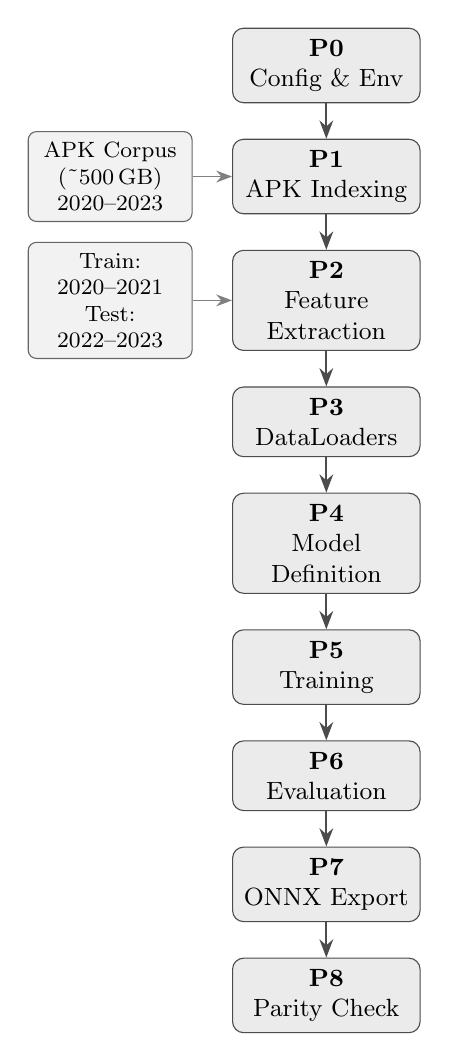
\begin{tikzpicture}[
					font=\small,
					>=Stealth,
					phase/.style={
						rectangle, rounded corners=4pt,
						draw=black!70, fill=black!8,
						text width=2.1cm, align=center,
						minimum height=0.75cm, inner sep=4pt
					},
					output/.style={
						rectangle, rounded corners=3pt,
						draw=black!60, fill=black!5,
						text width=1.8cm, align=center,
						minimum height=0.65cm, inner sep=4pt,
						font=\footnotesize
					},
					arr/.style={->, thick, black!70},
					sarr/.style={->, semithick, black!50},
					label/.style={font=\tiny\itshape, black!60}
					]
					%% ─── COLUMN 1 ONLY: PC OFFLINE PIPELINE ──────────────────────────────────
					\node[phase] (p0) at (0,0)     {\textbf{P0}\\Config \& Env};
					\node[phase, below=0.45cm of p0] (p1) {\textbf{P1}\\APK Indexing};
					\node[phase, below=0.45cm of p1] (p2) {\textbf{P2}\\Feature Extraction};
					\node[phase, below=0.45cm of p2] (p3) {\textbf{P3}\\DataLoaders};
					\node[phase, below=0.45cm of p3] (p4) {\textbf{P4}\\Model Definition};
					\node[phase, below=0.45cm of p4] (p5) {\textbf{P5}\\Training};
					\node[phase, below=0.45cm of p5] (p6) {\textbf{P6}\\Evaluation};
					\node[phase, below=0.45cm of p6] (p7) {\textbf{P7}\\ONNX Export};
					\node[phase, below=0.45cm of p7] (p8) {\textbf{P8}\\Parity Check};
					
					\draw[arr] (p0)--(p1); \draw[arr] (p1)--(p2); \draw[arr] (p2)--(p3);
					\draw[arr] (p3)--(p4); \draw[arr] (p4)--(p5); \draw[arr] (p5)--(p6);
					\draw[arr] (p6)--(p7); \draw[arr] (p7)--(p8);
					
					\node[output, left=0.5cm of p1] (corpus)
					{APK Corpus\\(\textasciitilde500\,GB)\\2020--2023};
					\draw[sarr] (corpus) -- (p1);
					\node[output, left=0.5cm of p2] (split)
					{Train: 2020--2021\\Test: 2022--2023};
					\draw[sarr] (split) -- (p2);
					% Columns 2 and 3 intentionally omitted: export bundle and model-family tiers
					% are described in the text and summarized in the experimental tables.
				\end{tikzpicture}%
			}
			\vspace{0.3em}
			\centerline{\footnotesize\textbf{(a) Offline pipeline}}
		\end{minipage}
		\hfill
		\begin{minipage}[t]{0.45\columnwidth}
			\centering
			\resizebox{\linewidth}{!}{%
				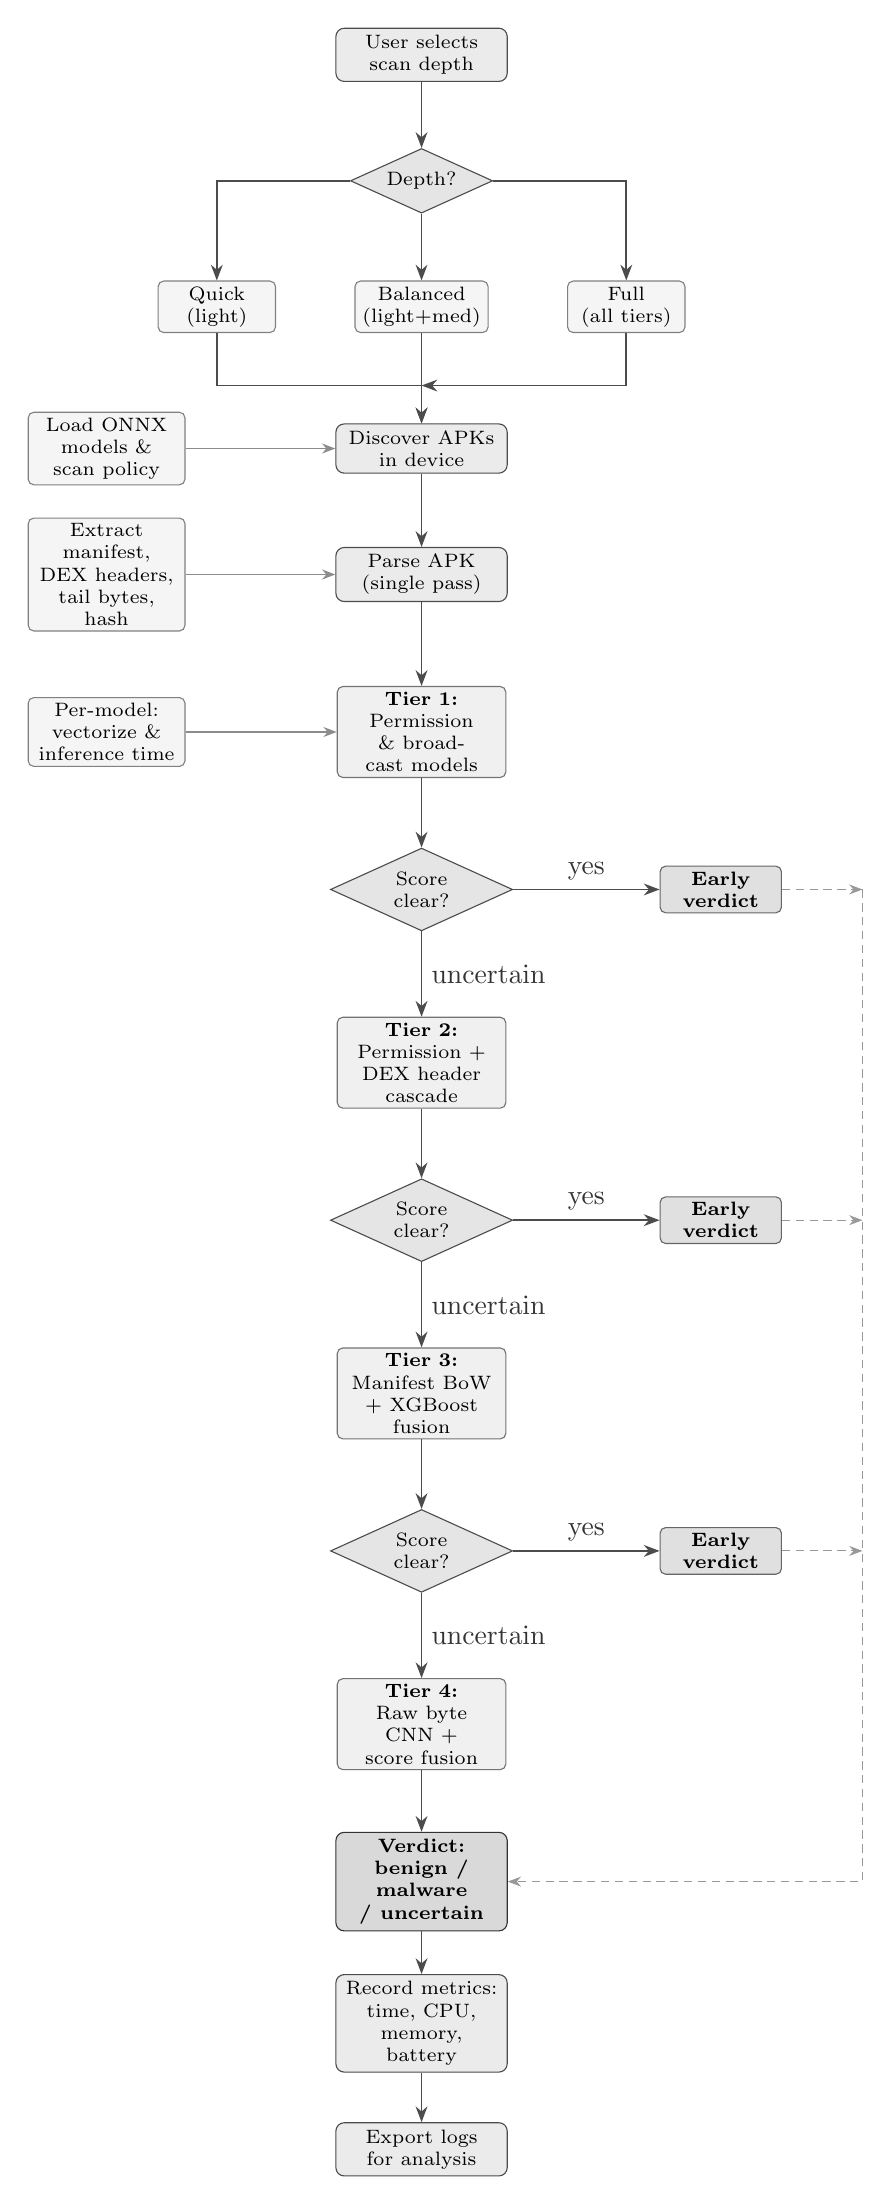
\begin{tikzpicture}[
					font=\scriptsize,
					>=Stealth,
					main/.style={
						rectangle, rounded corners=3pt,
						draw=black!70, fill=black!8,
						text width=2.0cm, align=center,
						minimum height=0.58cm, inner sep=2.5pt
					},
					decision/.style={
						diamond, aspect=2.2,
						draw=black!70, fill=black!10,
						text width=1.1cm, align=center,
						inner sep=1pt
					},
					verdict/.style={
						rectangle, rounded corners=3pt,
						draw=black!80, fill=black!15,
						text width=2.0cm, align=center,
						minimum height=0.55cm, inner sep=2.5pt,
						font=\scriptsize\bfseries
					},
					side/.style={
						rectangle, rounded corners=2pt,
						draw=black!50, fill=black!4,
						text width=1.85cm, align=center,
						minimum height=0.5cm, inner sep=2pt
					},
					tiernode/.style={
						rectangle, rounded corners=2pt,
						draw=black!55, fill=black!6,
						text width=2.0cm, align=center,
						minimum height=0.5cm, inner sep=2pt
					},
					exitnode/.style={
						rectangle, rounded corners=2pt,
						draw=black!60, fill=black!12,
						text width=1.4cm, align=center,
						minimum height=0.42cm, inner sep=2pt,
						font=\scriptsize\bfseries
					},
					arr/.style={->, semithick, black!70},
					sarr/.style={->, thin, black!45},
					darr/.style={->, densely dashed, thin, black!40},
					lbl/.style={font=\scriptsize, black!60}
					]
					
					%% ── Top: user interaction ────────────────────────────────────────────
					\node[main] (ui) at (0, 0.0) {User selects\\scan depth};
					\node[decision] (depth) at (0, -1.6) {Depth?};
					
					\node[side, text width=1.35cm] (dq) at (-2.6, -3.2) {Quick\\(light)};
					\node[side, text width=1.55cm] (db) at ( 0.0, -3.2) {Balanced\\(light+med)};
					\node[side, text width=1.35cm] (df) at ( 2.6, -3.2) {Full\\(all tiers)};
					\draw[arr] (ui) -- (depth);
					\draw[arr] (depth.west) -| (dq.north);
					\draw[arr] (depth.south) -- (db.north);
					\draw[arr] (depth.east) -| (df.north);
					%% ── Merge to scan ───────────────────────────────────────────────────
					\node[main] (scan) at (0, -5.0) {Discover APKs\\in device};
					\draw[arr] (dq.south) -- (-2.6, -4.2) -- (0, -4.2) -- (scan.north);
					\draw[arr] (df.south) -- ( 2.6, -4.2) -- (0, -4.2);
					\draw[arr] (db.south) -- (scan.north);
					
					%% ── Parse once ──────────────────────────────────────────────────────
					\node[main] (parse) at (0, -6.6) {Parse APK\\(single pass)};
					\draw[arr] (scan) -- (parse);
					%% ── Tier 1 ──────────────────────────────────────────────────────────
					\node[tiernode] (t1) at (0, -8.6) {
						\textbf{Tier 1:} Permission\\
						\& broadcast models
					};
					\draw[arr] (parse) -- (t1);
					%% ── Left annotations — properly spaced out ──────────────────────────
					\node[side] (rscan) at (-4.0, -5.0) {
						Load ONNX\\
						models \&\\
						scan policy
					};
					\draw[sarr] (rscan.east) -- (scan.west);
					
					\node[side] (fctx) at (-4.0, -6.6) {
						Extract manifest,\\
						DEX headers,\\
						tail bytes, hash
					};
					\draw[sarr] (fctx.east) -- (parse.west);
					\node[side] (rmetric) at (-4.0, -8.6) {
						Per-model:\\
						vectorize \&\\
						inference time
					};
					\draw[sarr] (rmetric.east) -- (t1.west);
					%% ── Tier Decisions — Deep vertical gaps for arrows ──────────────────
					\node[decision] (d1) at (0, -10.6) {Score\\clear?};
					\draw[arr] (t1) -- (d1);
					\node[exitnode] (e1) at (3.8, -10.6) {Early\\verdict};
					\draw[arr] (d1.east) -- node[above, font=\normalsize, black!80] {yes} (e1.west);
					%% ── Tier 2 ──────────────────────────────────────────────────────────
					\node[tiernode] (t2) at (0, -12.8) {
						\textbf{Tier 2:} Permission +\\
						DEX header cascade
					};
					\draw[arr] (d1.south) -- node[right, font=\normalsize, black!80] {uncertain} (t2.north);
					
					\node[decision] (d2) at (0, -14.8) {Score\\clear?};
					\draw[arr] (t2) -- (d2);
					\node[exitnode] (e2) at (3.8, -14.8) {Early\\verdict};
					\draw[arr] (d2.east) -- node[above, font=\normalsize, black!80] {yes} (e2.west);
					%% ── Tier 3 ──────────────────────────────────────────────────────────
					\node[tiernode] (t3) at (0, -17.0) {
						\textbf{Tier 3:} Manifest BoW\\
						+ XGBoost fusion
					};
					\draw[arr] (d2.south) -- node[right, font=\normalsize, black!80] {uncertain} (t3.north);
					
					\node[decision] (d3) at (0, -19.0) {Score\\clear?};
					\draw[arr] (t3) -- (d3);
					\node[exitnode] (e3) at (3.8, -19.0) {Early\\verdict};
					\draw[arr] (d3.east) -- node[above, font=\normalsize, black!80] {yes} (e3.west);
					%% ── Tier 4 ──────────────────────────────────────────────────────────
					\node[tiernode] (t4) at (0, -21.2) {
						\textbf{Tier 4:} Raw byte\\
						CNN + score fusion
					};
					\draw[arr] (d3.south) -- node[right, font=\normalsize, black!80] {uncertain} (t4.north);
					
					%% ── Final verdict ───────────────────────────────────────────────────
					\node[verdict] (verd) at (0, -23.2) {
						Verdict:\\
						benign / malware\\
						/ uncertain
					};
					\draw[arr] (t4) -- (verd);
					
					%% ── Early-exit dashed arrows ────────────────────────────────────────
					\draw[darr] (e1.east) -- (5.6, -10.6);
					\draw[darr] (e2.east) -- (5.6, -14.8);
					\draw[darr] (e3.east) -- (5.6, -19.0);
					\draw[darr] (5.6, -10.6) -- (5.6, -23.2) -- (verd.east);
					%% ── Metrics logging ────────────────────────────────────────────────
					\node[main] (log) at (0, -25.0) {
						Record metrics:\\
						time, CPU,\\
						memory, battery
					};
					\draw[arr] (verd) -- (log);
					\node[main] (export) at (0, -26.6) {
						Export logs\\
						for analysis
					};
					\draw[arr] (log) -- (export);
					
				\end{tikzpicture}%
			}
			\vspace{0.3em}
			\centerline{\footnotesize\textbf{(b) VigiDroid app flow}}
		\end{minipage}
		\caption{Proposed VigiDroid methodology.
			\textit{Left:} the offline model-development pipeline, with export and model-family details omitted for compactness.
			\textit{Right:} the on-device scan pipeline that selects a scan depth, extracts features locally, runs ONNX inference, fuses scores, and exports resource metrics.}
		\label{fig:methodology}
	\end{figure}
	
	
	
	
	
	
	
	\section{Experiments}
	
	\begin{table*}[t]
		\caption{Experimental comparison of on-device malware detection models.
			Offline metrics are computed on the computer temporal test split;
			resource columns are derived from on-device \texttt{all\_scan\_metrics.json}.}
		\label{tab:results}
		\centering
		\scriptsize
		\setlength{\tabcolsep}{8pt}
		\begin{tabular}{@{}l p{3.7cm} c c c c c c c c@{}}
			\toprule
			\textbf{Model} & \textbf{Features} & \textbf{Acc.} & \textbf{F1} & \textbf{ROC-AUC} & \textbf{CPU} & \textbf{Mem.} & \textbf{Batt.} & \textbf{Time} & \textbf{Feasible} \\
			\midrule
			XGBoost & Manifest perms, intents, APIs & 0.9372 & 0.8884 & 0.9913 & 97.4 ms & 0.02 MB & 477.102 & 100.0 ms & low \\
			1D-CNN & Last 1024 APK bytes & 0.9005 & 0.8486 & 0.9592 & 1.7 ms & 0.01 MB & 8.433 & 1.7 ms & low \\
			MLP-H & Dex header, sum-pooled & 0.9686 & 0.9478 & 0.9675 & 0.7 ms & 0.01 
			MB & 1.997 & 0.4 ms & high \\
			Dex+Manifest ASCNN & Dex header + manifest BoW & 0.9411 & 0.9064 & 0.9685 & 7.8 ms & 0.03 MB & 36.045 & 7.9 ms & medium \\
			Dex+Manifest Dual & Dex header + manifest, dual-branch & 0.9686 & 0.9483 & 0.9805 & 7.9 ms & 0.02 MB & 36.84 & 7.9 ms & medium \\
			LinRegDroid & Manifest permission flags & 0.9175 & 0.8645 & 0.9259 & 1.0 ms & 0.00 MB & 3.008 & 0.7 ms & low \\
			MLDP-pruned & MLDP-selected permissions & 0.9319 & 0.8855 & 0.9017 & 0.6 ms & 
			0.00 MB & 1.61 & 0.4 ms & medium \\
			Broadcast+MLDP & MLDP perms + receiver actions & 0.9359 & 0.8928 & 0.9373 & 1.1 ms & 0.00 MB & 1.76 & 0.4 ms & medium \\
			MLDP+Dex Cascade & MLDP perms + dex header & 0.9581 & 0.9298 & 0.9469 & 0.8 ms & 0.01 MB & 4.919 & 0.4 ms & high \\
			Dex+Broadcast Fusion & Dex header + receiver actions & 0.9699 & 0.9503 & 0.9794 & 0.9 ms & 0.01 MB & 2.362 & 0.5 ms & high \\
			Droidcat & 0.9739& 0.9739& \\
			\bottomrule
		\end{tabular}
	\end{table*}
	
	
	
	
	
	
	
	
	
	We evaluate each model in terms of 
	detection performance (Accuracy, F1-score, ROC-AUC on a temporal holdout set from 2022-2023) and on-device feasibility (CPU time, memory usage, battery consumption, and inference latency measured on a physical Android device).
	Table \ref{tab:results} summarizes the results obtained using VigiDroid under full-scan mode.
	Among all configurations, Dex+Broadcast Fusion achieved the best overall performance with 96.99\% accuracy and 0.9503 F1-score while requiring less than 1 ms inference time and negligible memory overhead.
	In contrast, API-based models such as XGBoost incurred substantially higher processing costs due to feature extraction overhead despite competitive detection performance.
	While prior approaches such as SeqMobile and DroidCAT reported higher detection accuracy, their reliance on sequence processing or behavioral analysis introduces significant computational overhead, limiting their practicality for real-time on-device deployment.
	\begin{figure}[H]
		\centering
		
\includegraphics[width=0.75\linewidth]{inferenceTime_vs_apkSize.png}
		\caption{Inference time vs APK size. Though inference time stays flat across APK sizes for all models, the cost is driven almost entirely by the feature domain, not the APK size itself.
		}
	\end{figure}
	
	
	
	
	
	\begin{figure}[H]
		\centering
		
\includegraphics[width=0.75\linewidth]{sample_model_vs_accuracy_resources.png}
		\caption{ This figure visualises trade-off directly: DEX-header-based models cluster in the high-accuracy, low-resource corner of the plot, while XGBoost sits isolated at high resource cost.}
		\label{fig:tradeoff}
	\end{figure}
	
	%\textbf{Detection quality.} The results span a meaningful range.
	At the top end, Dex+Broadcast Fusion achieves the highest accuracy (96.99\%) and F1 (0.9503) among all models, closely followed by MLP-H and the Dex+Manifest Dual model, both reaching 96.86\% accuracy.
	XGBoost posts the strongest ROC-AUC at 0.9913, reflecting its ability to rank samples well across thresholds, though its flat accuracy and F1 are more modest (93.72\% and 0.8884 respectively).
	Permission-only models like LinRegDroid and MLDP-pruned sit at the lower end of the accuracy range (91--93\%), confirming that richer structural features yield better discrimination.
	%\textbf{On-device cost.} The resource gap between models is striking. XGBoost consumes 97.4\,ms of CPU time and 477 battery units per scan — roughly two orders of magnitude more than the cheapest models — placing it in the low-feasibility category despite its strong ROC-AUC.
	The 1D-CNN similarly draws more resources than its accuracy warrants (1.7\,ms CPU, 8.4 battery units) for only 90.05\% accuracy.
	In contrast, the DEX-header family proves highly efficient: MLP-H, MLDP+Dex Cascade, and Dex+Broadcast Fusion all complete inference in 0.4--0.5\,ms with under 5 battery units consumed.
	These three are rated high feasibility in Table~\ref{tab:results}.
	%\textbf{Feature representation as the key variable.} 
	%Fig.~\ref{fig:inference time vs apk size} shows that inference time stays flat across APK sizes for all models — the cost is driven almost entirely by the feature domain, not the APK size itself.
	%Manifest-token models like XGBoost pay a high parsing cost because they must tokenize and aggregate across all \texttt{classes*.dex} files, whereas DEX header models extract a fixed 104-dimensional vector regardless of app complexity.
	%Fig.~\ref{fig:tradeoff}  This pattern holds consistently across CPU, memory, and battery metrics, suggesting that the feature extraction pipeline — not the classifier on top of it — is the primary bottleneck for on-device deployment.
	%\textbf{Protocol.} 
	%\textbf{Protocol (planned).}
	%Labeled eval APKs (\texttt{eval\_XXXX\_benign/malware.apk}) on device; metrics pulled via ADB; offline labels from corpus year splits.
	\section{Conclusion}
	We described VigiDroid, a thesis framework for practical on-device Android malware pre-screening that unifies literature-based static detectors through a disciplined train-export-deploy pipeline and tiered ONNX orchestration on Android.
	The results show that DEX-header-based models offer the best of both worlds, with Dex+Broadcast Fusion reaching 96.99\% accuracy and an F1 of 0.9503 while consuming under 1\,ms of CPU and 2.4 battery units per scan.
	At the other extreme, XGBoost's ROC-AUC of 0.9913 comes at the cost of 97.4\,ms CPU and 477 battery units.
	Across all models, the feature extraction pipeline proved to be the dominant cost factor, not the classifier architecture itself.
	%We believe this finding has practical implications for how future work in mobile malware detection should be designed and evaluated: deployment cost should be treated as a first-class constraint from the start, not measured as an afterthought.
	\section*{Acknowledgment}
	The authors thank their supervisor and collaborators at the Department of Computer Science and Engineering, BUET, for guidance throughout this thesis.
	\begin{thebibliography}{00}
		\bibitem{bytecnn}
		C.~Hasegawa and H.~Iyatomi,
		``One-dimensional convolutional neural networks for Android malware detection,''
		in \textit{Proc.\ ICCE}, 2020.
		
		\bibitem{linregdroid}
		A.~Narayanan et al.,
		``LinRegDroid: Detection of Android malware using multiple linear regression,''
		\textit{Computers \& Security}, 2018.
		\bibitem{msdroid}
		Tao Peng et al.,
		``A Lightweight Multi-Source Fast Android Malware Detection Model,''
		\textit{Appl.
			Sci.}, 2022.
		
		
		\bibitem{broadcast}
		M.~Mohsen and A.~Ismail,
		``Detecting Android malwares by mining statically registered broadcast receivers,''
		\textit{Int.\ J.\ Advanced Computer Science and Applications}, 2017.
		\bibitem{seqmobile}
		Ruitao Feng et al.,
		``SeqMobile: An Efficient Sequence-Based Malware Detection System Using RNN on Mobile Devices''
		\textit{ 25th International Conference on Engineering of Complex Computer Systems (ICECCS)}, 2020.
		\bibitem{samadroid}
		Saba Arshad et al.,
		``SAMADroid: A Novel 3-Level Hybrid Malware Detection Model for Android Operating System''
		\textit{IEEE Access}, 2018.
		\bibitem{dldroid}
		Mohammed K. Alzaylaee et al.,
		``DL-Droid: Deep learning based android malware detection using real devices''
		\textit{IEEE Access}, 2020.
		
		\bibitem{mldp}
		S.~Wang et al.,
		``Permission extraction framework for Android malware detection,''
		\textit{IEEE Access}, 2019.
		
		\bibitem{msfdroid}
		Y.~Li et al.,
		``MSFDroid: Multi-stage fusion for Android malware detection,''
		\textit{IEEE Trans.\ Information Forensics and Security}, 2022.
		\bibitem{mh1m}
		Bragança, H., 
		Kreutz, D., Rocha, V. et al. ,
		``MH-1M: A 1.34 Million-Sample Multi-Feature Android Malware Dataset with Rich Metadata.,''
		\textit{Sci Data 13, 153 .
			https://doi.org/10.1038/s41597-025-06469-5}, 2026.
		\bibitem{msfdroid}
		Tao Peng et al.,
		``A Lightweight Multi-Source Fast Android Malware Detection Model,''
		\textit{Appl.
			Sci.}, 2022.
		\bibitem{drebin}
		D.~Arp et al.,
		``Drebin: Effective and explainable detection of Android malware in your pocket,''
		in \textit{Proc.\ NDSS}, 2014.
		
		\bibitem{onnx}
		ONNX Runtime documentation,
		\url{https://onnxruntime.ai/}, accessed 2026.
	\end{thebibliography}
	
	
	
	
\end{document}